\documentclass[a4paper,12pt]{article}
\usepackage{graphicx}
\usepackage{titlesec}
\usepackage[utf8]{inputenc}
\usepackage{xcolor}
\usepackage{fancyhdr}
\usepackage{lipsum}
\usepackage{caption}

\renewcommand{\headrulewidth}{0pt}
\fancyhead[C]{}
\fancyhead[C]{
	
\includegraphics[width=4cm]{metu}
}
\pagestyle{plain}

%opening
\title{Middle East Technical University\\Department of Physics\\\textbf{PHYS307 Applied Modern Physics}}
\author{Oğuzhan ÖZCAN\\}
\date{}
\clearpage
\thispagestyle{empty}
\providecommand{\groupmember}[1]{\textbf{Group Members:} }
\providecommand{\expdate}[1]{\textbf{Experiment Date:} }
\providecommand{\repdate}[1]{\textbf{Report Submit Date:} }
\providecommand{\expname}[1]{\textbf{Exp. MP-ED The Diffraction of Electrons by Graphite} }


\usepackage[a4paper,%
left=0.5in,right=0.5in,top=0.5in,bottom=0.8in,%
footskip=.25in]{geometry}
%\topmargin -4.5cm
%\oddsidemargin 0.2cm
%\textwidth 16cm %
%\textheight 21cm%
%\footskip 1.0cm%




\begin{document}
\pagenumbering{gobble}
\maketitle

\thispagestyle{fancy}

%%%%%%%%%%%%%%%%%%%%%%%%%%%%%%%%%%%%%%%%%%%%%%%%%%%%%
\noindent\rule{18.4cm}{0.8pt}
\begin{center}
	\expname{arg1}{}
\end{center}

\expdate{November 6, 2015}{December 18, 2015}\\
\repdate{arg1}{December 25, 2015}\\
\noindent\rule{18.4cm}{0.8pt}\\\\
%%%%%%%%%%%%%%%%%%%%%%%%%%%%%%%%%%%%%%%%%%%%%%%%%%%%%
\begin{figure}[h!]
\centering
\includegraphics[scale = 0.9]{"table 1"}
\caption{Data for the first two interference rings on the diffraction pattern}
\label{fig:table1}
\end{figure}

\textbf{Lattice Constants:}
\begin{center}
	$d_{1}=2.09 \pm 0.012 \AA{}$\\
    $d_{2}=1.20 \pm 0.048\AA{}$
\end{center}
In the laboratory manual graphite planes for the first two interference rings is given below:\\
\begin{center}
	$d_{1}=2.13 \AA{}$\\
	$d_{2}=1.23 \AA{}$
\end{center}
\newpage
\begin{figure}[h!]
\centering
\includegraphics[scale = 1.0]{"table 2"}
\caption{Latice constants for each voltage value }
\label{fig:table2}
\end{figure}
\textbf{1. What is the implication of the diffraction pattern on the screen in the experiment you have carried out?}\\\\
We targeted an electron gun to graphite planes as we mentioned in manual. When an electron strikes to graphite planes, it scatters an electron from this plate. After passing through from collimators we can see these electrons as a pattern on the screen. Theoretically we could have seen more than two circular line on the screen but we observed an electron beam at the center and two circular lines around this beam. Below figure illustrates the experiment. On the right figure, after second ring, circles started to blurred.\\\\
\begin{figure}[h!]
\centering
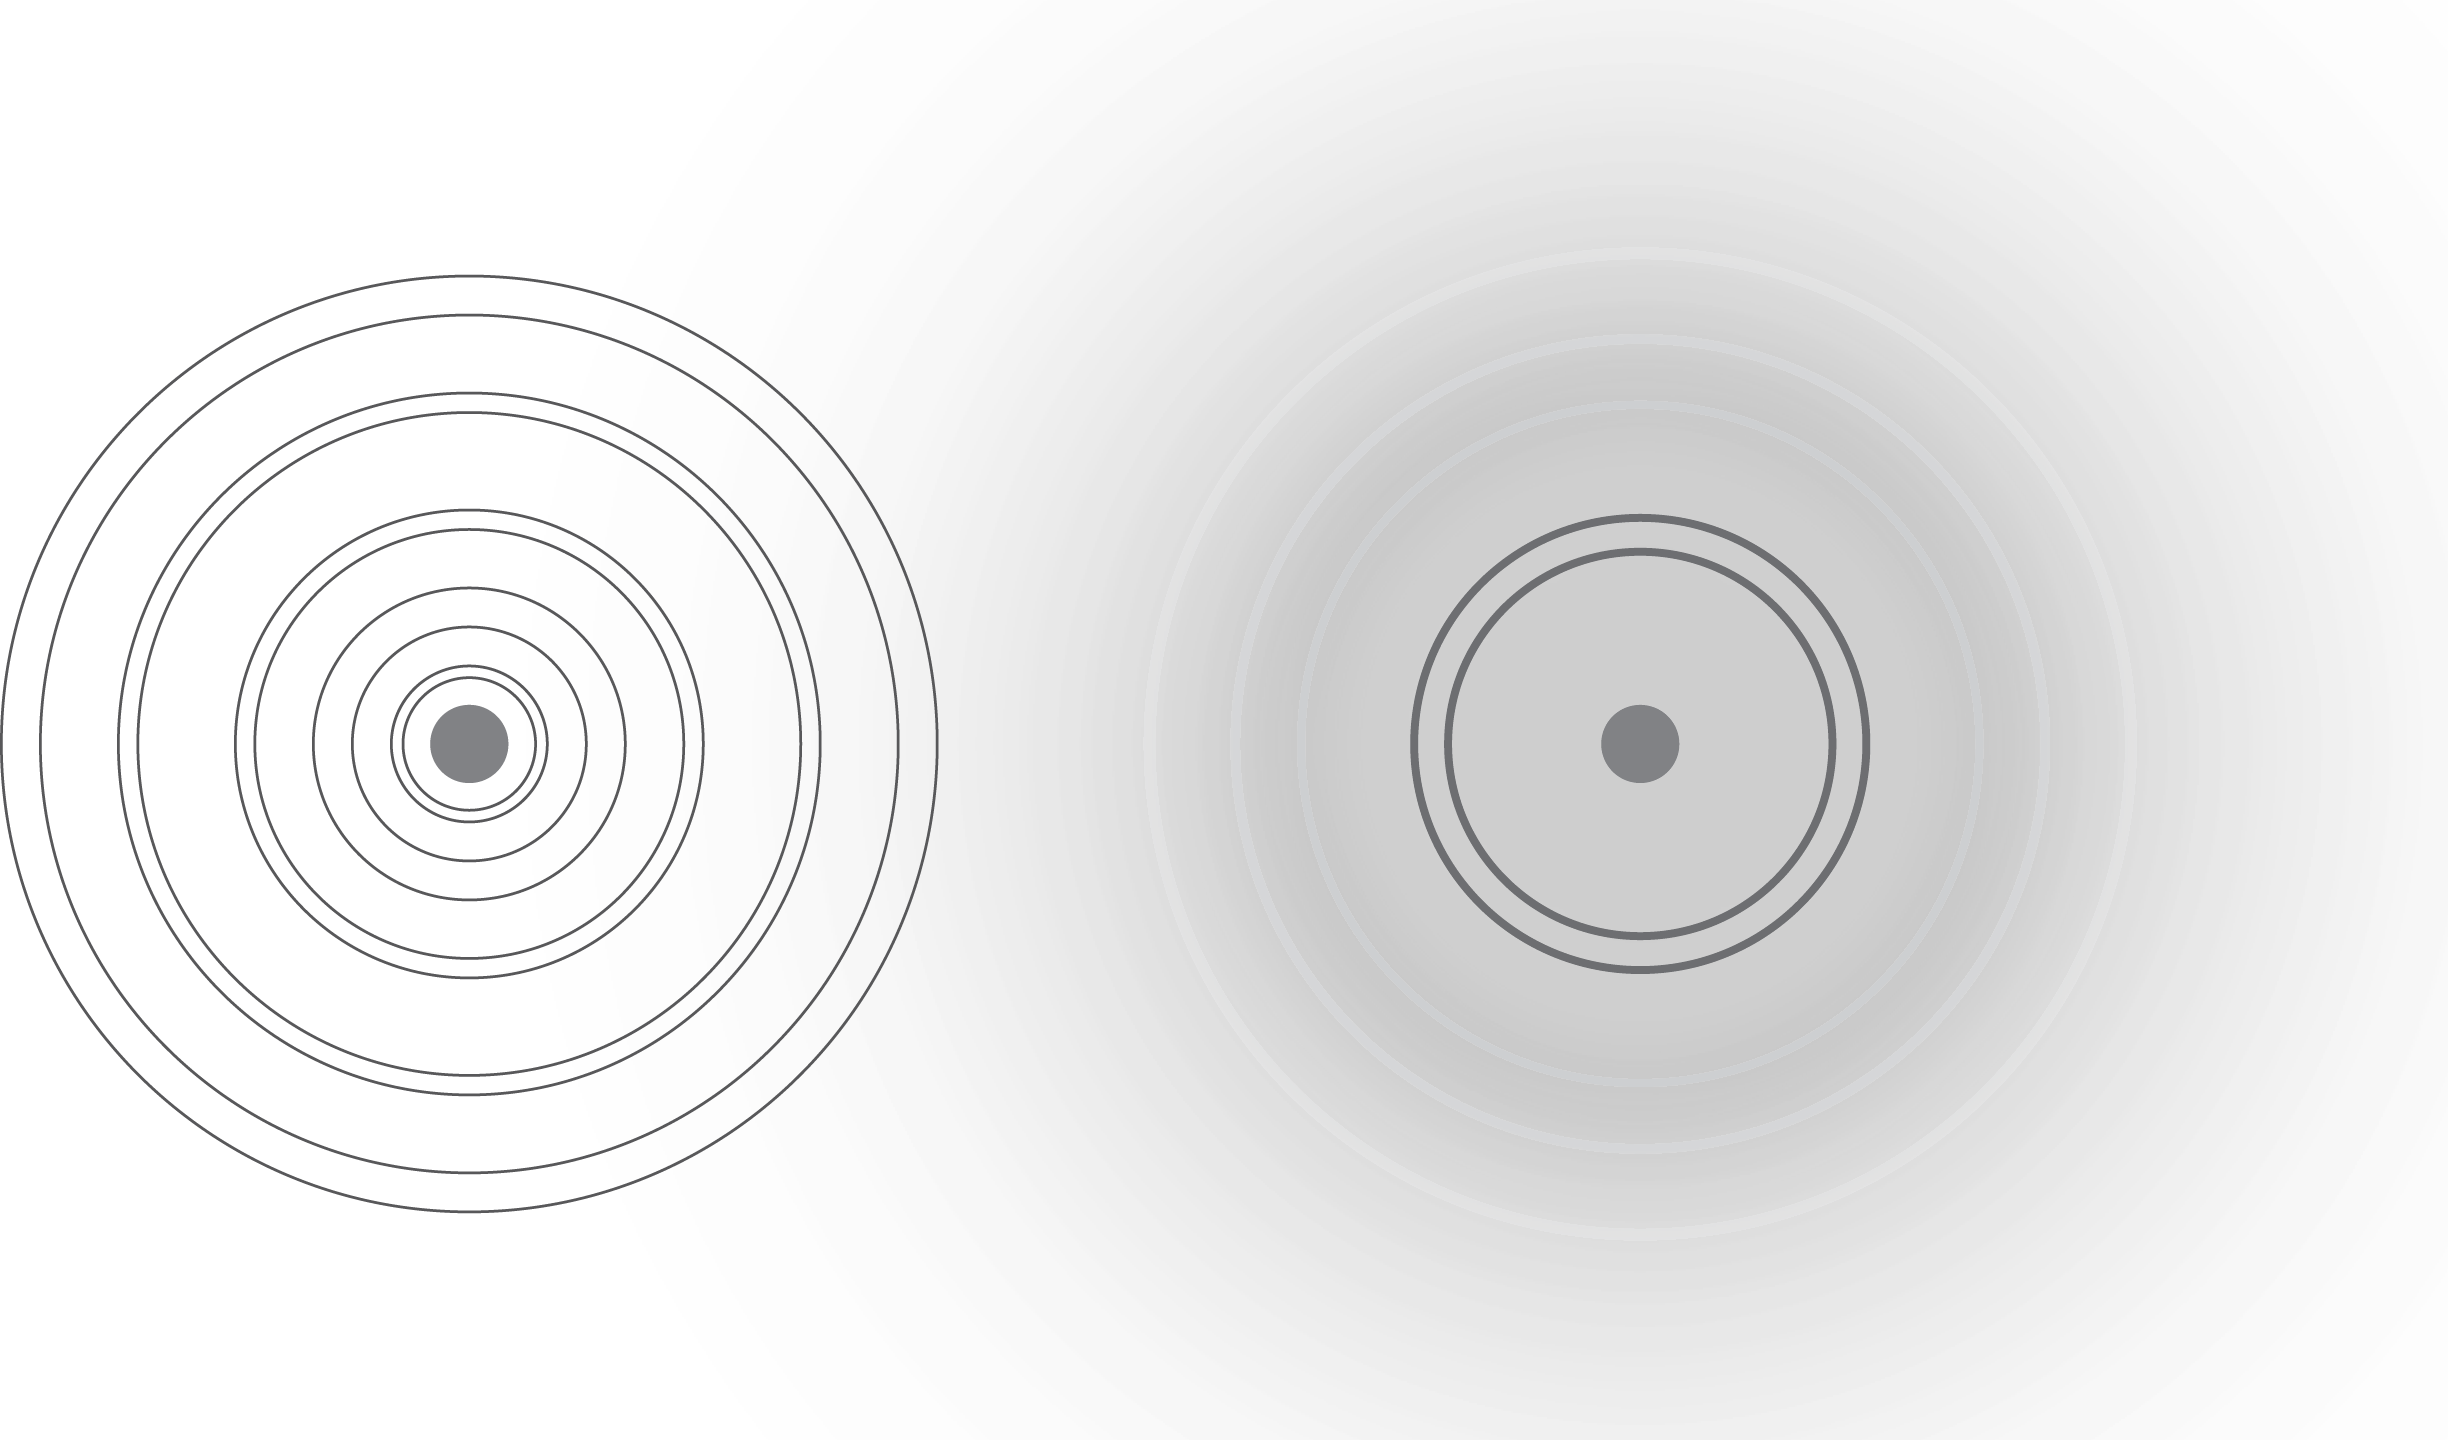
\includegraphics[scale = 0.65]{screen}
\caption{\textbf{Left:} Predicted screen resolution for diffraction pattern. \textbf{Right:} Observed screen resolution for diffraction pattern. }
\label{fig:screen}
\end{figure}
\newpage
\textbf{2. What properties of a material can be determined from the experiment you have carried out?}\\\\
We can determine the wavelength of electrons, verify the de Broglie's equation, determine the lattice place spacing of graphite and structure of crystal. If we have some solid state physics knowledge we can determine the type of crystals whether simple cubic, face-centered cubic or body-centered cubic. Since we measure the wavelength of material, we can also calculate mass, momentum and some other basic properties of related material.\\\\ 
\textbf{Discussion and Conclusion}\\\\
As we know, light can behave both particle and wave like. In this experiment we studied the wave behaviour of electrons. The wave aspect of particle first demonstrated by C. H. Davisson and L.H. Gerner. After this experiment, hypothesis of L. de Broglie is corrected he was awarded the Nobel Prize in Physics in 1929. In 1937, Davisson and Gerner received Nobel Prize for their experiment. In this experiment we used a crystal graphite to scatter electrons. As seen in Figure 3, we observed only two rings on the screen. Since this is not enough to determine a correct wavelength, we changed voltage and measured the differences in those rings. This difference can be seen in Figure 1. Theoretical values for lattice constants are mentioned above. By using them we can calculate a percentage error for this experiment:
\begin{equation}
Percentage Error=\frac{|Theoretial Value-Experimental Value|}{Theoretial Value}\times 100
\end{equation}
For $d_{1}$
\begin{equation}
Percentage Error=\frac{|2.13-2.09|}{2.13}\times 100 = \framebox[30pt]{1.9\%}
\end{equation}
For $d_{2}$
\begin{equation}
Percentage Error=\frac{|1.23-1.20|}{1.23}\times 100 = \framebox[30pt]{2.4\%}
\end{equation}
There is an extra table in this report as seen in Figure 2. Since we have different $d_{1}$ and $d_{2}$ values for each voltage and wavelength, I calculated an average value for them. These lattice constants are calculated according to following equation:
\begin{equation}
d=n \frac{2R}{r}\lambda
\end{equation}
where $R=0.0635$ m, $n=1$, $r$ and $d$ are varies according to Figure 1. We can say that this experiment is accomplished it is because we have very low percentage errors and we observed what we predict before the experiment. These errors caused by human falses and setup falses. For instance, as stated in manual setup reduces the voltage ratio 100:2.














































































































































\end{document}
